\chapter[SCP-084 静滞塔]{
    SCP-084 Static Tower\\
    SCP-084 静滞塔
}

\label{chap:SCP-084}

\begin{figure}[H]
    \centering
    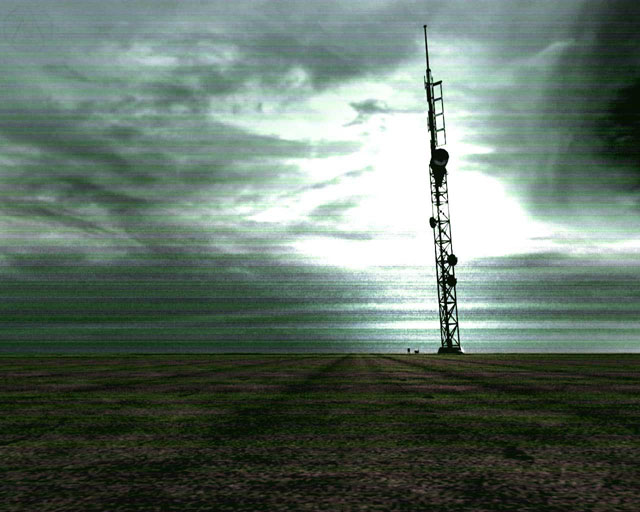
\includegraphics[width=0.5\linewidth]{images/SCP.084.jpg}
    \caption*{SCP-084。从首次侦察记录中获得的图像。所有其它图像均被SCP-084的“广播”扰乱。}
\end{figure}

\bb{项目编号:}SCP-084

\bb{项目等级:}Euclid

\bb{特殊收容措施:}当前命令全面禁止在估计出辐射波的范围之前与SCP-084互动(关于一般的全面禁止互动命令的详细记载参见文档XRG-1182;关于与SCP-084相关的全面禁止互动命令的详细记载参见文档XRG-1208A)。应持续监控SCP-084作用区域周边,主要目的为误导平民和外部监视。由于附近没有重要道路、小径或其它旅游路线,遇到的任何接近SCP-084的平民均应被视为可疑对象并被拘留以待评估。任何情况下不允许基金会或平民人员进入SCP-084作用区域,除非得到至少两(2)名O5指挥部成员明确的口头和书面许可。

哨兵应保持原位不动,以视线检查其它哨兵,同时检查指南针和地标。所有参考点应远处于SCP-084的作用区域外侧。一旦有哨兵在点名时未报告情况,则召回所有哨兵,并由特别应对小组重新评估收容情况。若作用区域大小发生波动,所有在岗哨兵将执行召回命令,之后将采取合适的行动。

禁止一切形式的收音机、GPS、电视、手机、摄像机、照相机或任何其它记录或电子媒体设备进入距离SCP-084周边作用区域一百(100)米内。若在该范围内发现携带上述设备的平民,应立即没收并销毁其设备。收缴到的任何记录{[}数据删除]。

\bb{描述:}SCP-084外表是一个大型无线电塔,位于一大片开阔地,拥有两座小型附属建筑。由于SCP-084周围\slash 从SCP-084散发的影响,不可能对SCP-084进行直接观察和样品采集。SCP-084似乎发射一种对当地的时空\slash 现实产生不利影响的波或辐射。其最显著的效果是SCP-084作用区域内的空间变化。从外部看,作用区域大致呈一个直径二百(200)米的“圆顶”形。SCP-084在区域内的随机地点出现,\hyperref[chap:SCP-2675]{似乎在随机时刻“跳跃”},有时甚至在作用区域内的多个地点同时显现。从内部看,该空间似乎是无限大的,SCP-084位于其“中心”。

\begin{figure}[H]
    \centering
    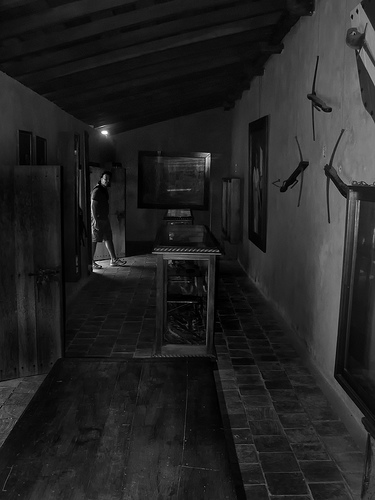
\includegraphics[width=0.5\linewidth]{images/SCP.084.2.jpg}
    \caption*{侦察小队B-3记录的图像。小队当时正对一条铺有地砖的空旷走廊拍照。}
\end{figure}

由于“散发出的影响”,不可能到达SCP-084。从作用区域内部接近SCP-084的尝试返回的汇报称即便在同时利用交通工具和双腿进行的三个月零十二天专心致志的直线行进之后,SCP-084仍保持其在地平线上的相对位置不变。已证实摧毁测试是不可能的,因为任何摧毁手段都无法在物理层面上接触SCP-084,甚至包括从作用区域外进行摧毁的情况。同时,当地空间会定期扭曲。这使得相对距离在“一闪”之间随机延长或缩短,导致建筑或物体突然“跳”到几千米之外,或“冲”到其它地点,有时甚至导致“重叠”。这种“重叠”对活体组织有显著的负面影响。

██████████ █████镇被认为曾位于最初成形的作用区域内或周边。这个镇已经无法从作用区域外部被观测,而是只在作用区域内出现。██████████ █████镇在封闭期间人口无变化(343人)。似乎不可能有新生儿,正常的年龄算法也不适用。自杀和\slash 或谋杀似乎会被该区域的效应规避:死者在死亡数秒后“闪烁”并无伤复活。同时,有关于事件“倒带”导致致命伤口看上去“定格”并愈合一类的事的报告。居民看上去表现出大量时空不一致事件,大部分建筑同样如此(详细观测结果参见日志084-A4)。

电子设备和记录仪器在作用区域内或周围无法正常运转。实验者报告从视、音频记录及播放设备中得到的是“极其怪异”或“令人不安”的信息。这使得██████████ █████与外界完全隔离开来,不必由基金会进行收容。而且,似乎经过一段长度不定的时间后就再也无法离开作用区域。一名来自██████████ █████的对象——在开阔地上被发现——称他已经旅行了六年。他在距离██████████ █████城区边界约四百米处被找到。

\hr

\hyperref[chap:DOC-log-084-a4]{日志084-A4}:观测到的SCP-084相关异常事件记录

\hr
